\chapter{PENDAHULUAN}

\section{Latar Belakang}

\emph{Non Fungible Token} (\emph{NFT}) adalah identitas digital yang tidak dapat diduplikasi, digantikan, dan dibagikan yang tersimpan di dalam \emph{blockchain} \parencite{BakerBradley}. 
Dengan karakteristiknya tersebut, \emph{NFT} dapat digunakan untuk memvalidasi orisinalitas dan kepemilikan seseorang atas aset digital tertentu. Pada awal kemunculannya \emph{NFT} banyak digunakan pada bidang untuk karya seni digital.  \emph{NFT} sendiri hanya merepresentasikan kepemilikan suatu aset digital tetapi tidak merepresentasikan hak intelektual atau hak cipta dari aset tersebut. 

Dalam perkembangannya \emph{NFT} mengalami perubahan bentuk dari yang awalnya berupa gambar 2 dimensi menjadi 3 dimensi bahkan terdapat NFT dalam bentuk audio dan juga file lain. 
Selain itu \emph{NFT} juga dimanfaatkan dalam hal lain selain dalam karya seni digital seperti contohnya pada \emph{game} dari \emph{game} yang sederhana hingga \emph{game} yang mengusung konsep \emph{metaverse}. Istilah \emph{Metaverse} sendiri merupakan konsep dunia berbasiskan 3D \emph{virtual reality} yang memungkinkan para pengguna dapat saling terhubung, berkomunikasi, beraktivitas bersama, hingga melakukan kegiatan ekonomi layaknya di dunia nyata \parencite{YohanHwang}. 
Dalam praktiknya para pengguna akan memiliki \emph{avatar} sebagai representasi mereka di \emph{metaverse}, seluruh data akan disimpan ke dalam jaringan \emph{blockchain}, mata uang yang berlaku di \emph{metaverse} adalah \emph{cryptocurrency}, dan barang-barang yang ada pada \emph{metaverse} pada dasarnya adalah suatu NFT.

Meskipun menghadirkan berbagai potensi keuntungan, \emph{NFT Markeplace} yang awalnya digunakan lebih sebagai \emph{platform} jual beli karya seni digital masih memiliki berbagai keterbatasan dalam implementasinya sebagai \emph{platform} jual beli dari \emph{game} yang mengusung konsep \emph{metaverse}. Hal ini dikarenakan masih minimnya kemampuan integrasi dengan \emph{platform} luar sehingga mengakibatkan potensi penggunaan dan kemanfaatan dari \emph{NFT} menjadi tidak optimal. Mayoritas \emph{game} yang mengusup konsep \emph{metaverse} seperti \emph{The Sandbox} dan \emph{Decentraland} mengembangkan \emph{NFT marketplace} mereka sendiri. 
Selain itu, \emph{NFT marketplace} yang ada saat ini memiliki masih sangat terbatas dengan implementasi fungsi-fungsi dasar yang disediakan oleh \emph{smart contract} ERC-721 sehingga menyebabkan potensi penggunaan dan keuntungan \emph{NFT} atas suatu kepemilikan aset juga tidak maksimal. Contoh konkretnya adalah pemilik hanya dapat memperoleh keuntungan melalui penjualan asetnya. 
Hal ini tentunya berbeda dengan kepemilikan aset di dunia nyata dimana pemilik dapat memperoleh keuntungan dengan menyewakan aset yang dimiliki atau bahkan menjual sebagian kepemilikannya dengan orang lain.
Tentunya hal ini bertentangan dengan konsep \emph{metaverse} yang berupaya untuk membawa pengalaman di dunia nyata semirip mungkin ke dunia digital. 
Dengan fitur yang masih sederhana ini menyebabkan likuiditas dari \emph{NFT} sebagai aset dalam \emph{metaverse} rendah dikarenakan hanya dapat diperjual belikan dan dimiliki kalangan tertentu. 
Likuiditas sendiri menjadi penting dikarenakan likuiditas merupakan salah satu faktor pembentukan harga aset tak terkecuali \emph{NFT} sebagai aset digital dalam \emph{metaverse}.  

\begin{figure} [H] \centering
  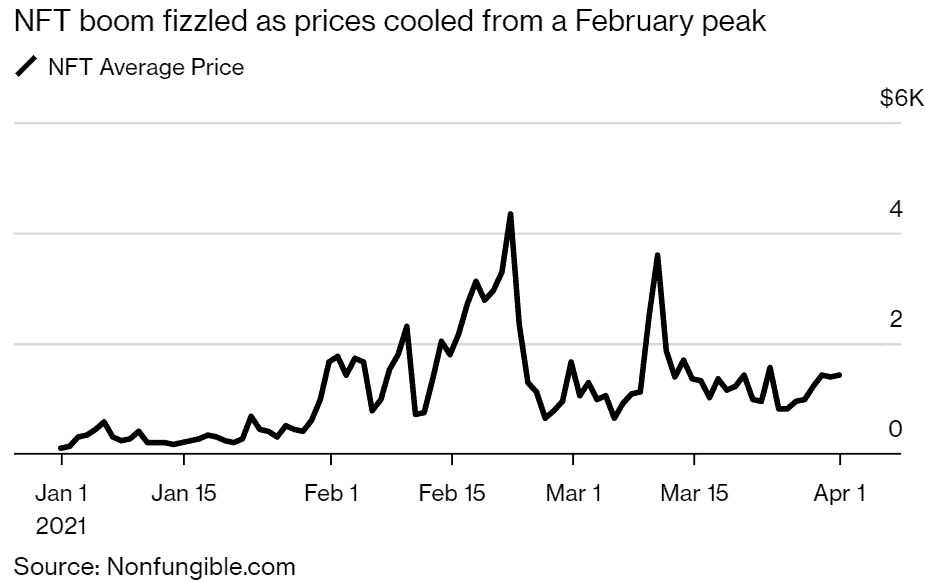
\includegraphics[scale=0.45]{gambar/img-nft-price-history.png}
  \caption{Pergerakan Harga NFT}
  \label{fig:Architecture}
\end{figure}

Grafik diatas merupakan salah satu contoh pergerakan harga rata-rata NFT dalam kurun waktu 4 bulan pada awal tahun 2021. Pada grafik tersebut terlihat bahwa pergerakan harga NFT cenderung fluktuatif, berbeda dengan aset layaknya di dunia nyata yang lebih stabil. Hal ini disebabkan oleh faktor potensi penggunaan dan keuntungan atas kepemilikan yang masih sangat minim yaitu hanya sebagai karya seni dan juga likuiditas yang rendah. 
Hal ini mengakibatkan pergerakan harganya tidak stabil dan hanya ditentukan oleh isu yang sedang tren di masyarakat.

Berangkat dari permasalahan tersebut penulis memiliki keinginan untuk mengembangkan suatu platform NFT marketplace yang memiliki fitur-fitur yang dapat memperluas potensi penggunaan \emph{NFT}, meningkatkan keuntungan atas kepemilikan NFT, dan meningkatkan likuiditas dari aset NFT sehingga dapat meningkatkan aspek ekonomi dari \emph{metaverse} layaknya di dunia nyata. 

\section{Rumusan Masalah}
Berdasarkan latar belakang yang telah dipaparkan dapat diketahui bahwa terdapat permasalahan pada penggunaan \emph{NFT} pada \emph{metaverse} disamping keuntungan yang diperoleh yaitu keterbatasan fitur \emph{NFT Marketaplce} sehingga mengakibatkan NFT yang digunakan sebagai aset dalam \emph{metaverse}
\begin{itemize}
  \item Kemampuan integrasi dengan platform lain yang terbatas
  \item Potensi penggunaan dan keuntungan atas kepemilikan \emph{NFT} yang tidak optimal
  \item Likuiditas yang rendah
  \item Harga yang tidak stabil
\end{itemize}

\section{Batasan Masalah atau Ruang Lingkup}

Adapun batasan masalah agar pembahasan topik ini dapat terarah dan mencapai tujuan. Batasan-batasan masalah tersebut adalah sebagai berikut:
\begin{enumerate}
  \item Pembuatan NFT marketplace berbasis \emph{blockchain} Ethereum.
  \item Target pengguna ialah seluruh pengguna yang terlibat dalam \emph{metaverse}.
  \item Pengujian transaksi dilakukan melalui jaringan \emph{Hardhat} sehingga penelitian berbentuk eksperimen, tidak menggunakan nominal real \emph{Ether}.
  \item Fitur yang akan dikembangkan pada NFT \emph{marketplace} ini adalah sistem sewa dan pembagian kepemilikan aset NFT.
\end{enumerate}

\section{Tujuan}

Berdasarkan permasalahan yang sudah dijelaskan, tujuan dari tugas akhir ini adalah untuk mengembangkan suatu platform \emph{NFT Marketplace} yang memiliki fitur sistem penyewaan NFT dan pembagian kepemilikan sehingga dapat meningkatan likuiditas aset dan aspek ekonomi dari suatu \emph{metaverse}.

\section{Manfaat}

\begin{enumerate}
  \item Bagi para pengguna \emph{metaverse} yaitu meningkatan potensi kemampuan pengguna untuk dapat menggunakan suatu aset bahkan memiliki suatu aset.
  \item Bagi para pengguna \emph{metaverse} yang memiliki aset NFT dapat meningkatan potensi keuntungan yang diperoleh dari aset yang dimiliki.
  \item Meningkatkan aspek ekonomi pada \emph{metaverse}.
\end{enumerate}
